\documentclass{article}

\usepackage{tikz-opm}
\usepackage{a4wide}
\usepackage{etoolbox}

\usepackage[T1]{fontenc}
\usepackage{dejavu}

\usepackage{showexpl}

\lstset{basicstyle=\ttfamily\small,
 explpreset={rframe={}}}

\usetikzlibrary{fit}


\begin{document}

\tikzset{every node/.style={font={\usefont{T1}{DejaVuSerifCondensed-TLF}{m}{n}}}}

\section{\texttt{tikz-opm}: creating Object Process Methodology diagrams with Tikz}
\label{sec:tikz-opm:-creating}



The \texttt{tikz-opm} package allows you to create nice OPM diagrams
using a number of relatively simple commands.

The package does not attempt to do any clever things - I am not
clever enough to encode smart placement of things like the aggregation
symbol below the object it applies to. Sorry.

But it does allow you to most of the important things from OPM
displayed in your diagram, so that is pretty good.



First we start out with the picture from the front of the OPM book:

\begin{LTXexample}[caption=OPM book front page,pos=t, varwidth=false]
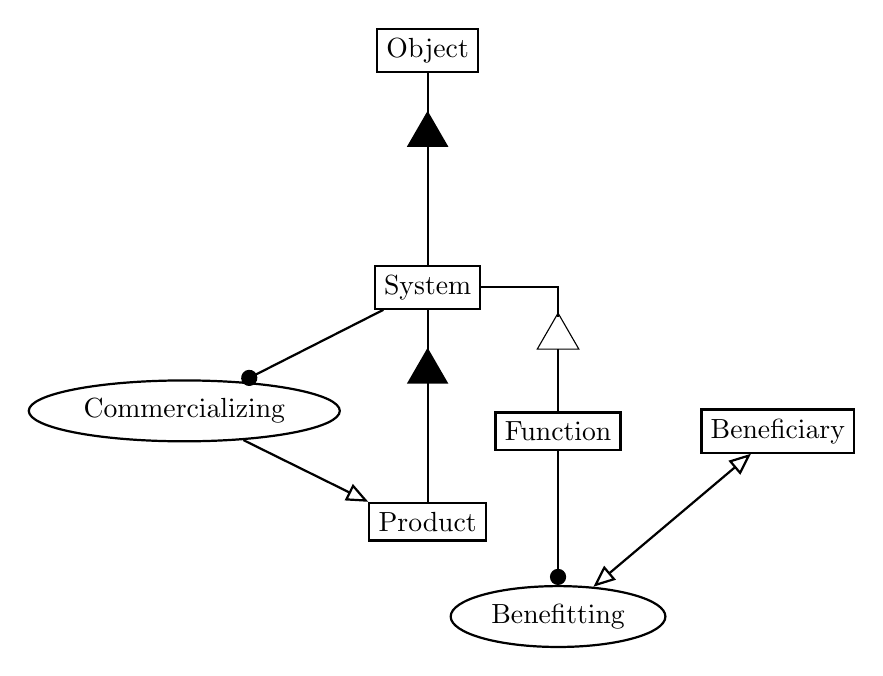
\begin{tikzpicture}
  \node [opmobject] (object) {Object};
  \node [opmaggregation, below=of object] (object-aggr) {};
  \path (object) edge (object-aggr);
  \node [opmobject, below=of object-aggr] (system) {System};
  \path (object-aggr) edge (system);
  \node [opmprocess, below left=of system] (commercializing)
  {Commercializing};
  \path (system) edge [opmagent] (commercializing);
  \node [opmaggregation, below=of system] (system-aggr) {};
  \node [opmobject, below=of system-aggr] (product) {Product};
  \path (system) edge (system-aggr) edge (product);
  \path (commercializing) edge[opmoutput] (product.north west);
  \node [opmgeneralization, below right=25pt of system, xshift=10pt] (system-gen) {};
  \node [opmobject, below=15pt of system-gen] (function) {Function};
  \draw [thick] (system.east) -| (system-gen.north);
  \path (system-gen.south) edge (function);
  \node [opmprocess, below=of function, yshift=-20pt] (benefitting) {Benefitting};
  \path (function) edge[opmagent] (benefitting);
  \node [opmobject, right=of function] (beneficiary) {Beneficiary};
  \path (benefitting) edge[opmeffect] (beneficiary);
\end{tikzpicture}
\end{LTXexample}

\section{Catalog of OPM symbols}
\label{sec:catalog-opm-symbols}

\lstset{
  explpreset={rframe={},width=0.3\linewidth}}


\begin{LTXexample}[rangeprefix=\%, rangesuffix=,
  includerangemarker=false, linerange=start-stop] 
  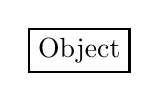
\begin{tikzpicture}
    %start
    \node [opmobject] (object) {Object};
    %stop
  \end{tikzpicture}
\end{LTXexample}


\begin{LTXexample}[rangeprefix=\%, rangesuffix=,
  includerangemarker=false, linerange=start-stop] 
  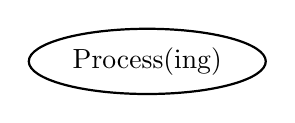
\begin{tikzpicture}
    %start
    \node [opmprocess] (processing) {Process(ing)};
    %stop
  \end{tikzpicture}
\end{LTXexample}

\begin{LTXexample}[rangeprefix=\%, rangesuffix=,
  includerangemarker=false, linerange=start-stop, caption=Aggregation
  for object, pos=t] 
  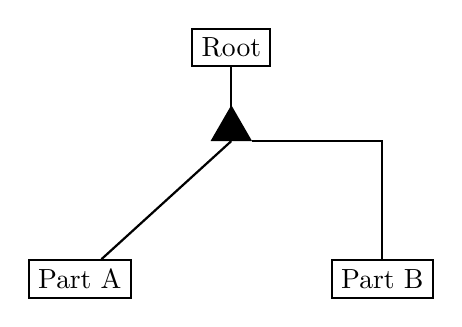
\begin{tikzpicture}
    %start
    \node [opmobject] (root) {Root};
    \node [opmaggregation, below=of root] (root-aggr) {};
    \path (root) edge (root-aggr);
    \node [opmobject, below left=of root-aggr] (part-a) {Part A};
    \node [opmobject, below right=of root-aggr] (part-b) {Part B};
    \path (root-aggr) edge (part-a);
    \draw [thick] (root-aggr.east) -| (part-b.north);
    %stop
  \end{tikzpicture}
\end{LTXexample}

Note that in order to get the more traditional vertial/horizontal
lines with right angles one has to use \verb|draw| and the \verb,-|,
operator. 

\begin{LTXexample}[rangeprefix=\%, rangesuffix=,
  includerangemarker=false, linerange=start-stop, pos=t,
  caption=Aggregation for process] 
  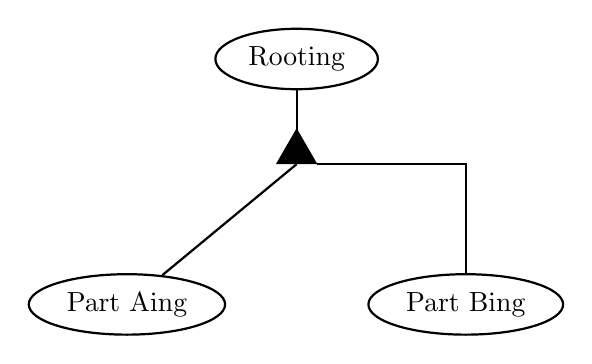
\begin{tikzpicture}
    %start
    \node [opmprocess] (root) {Rooting};
    \node [opmaggregation, below=of root] (root-aggr) {};
    \path (root) edge (root-aggr);
    \node [opmprocess, below left=of root-aggr] (part-a) {Part Aing};
    \node [opmprocess, below right=of root-aggr] (part-b) {Part Bing};
    \path (root-aggr) edge (part-a);
    \draw [thick] (root-aggr.east) -| (part-b.north);
    %stop
  \end{tikzpicture}
\end{LTXexample}

\begin{LTXexample}[rangeprefix=\%, rangesuffix=,
  includerangemarker=false, linerange=start-stop, pos=t,
  caption=Exhibition] 
  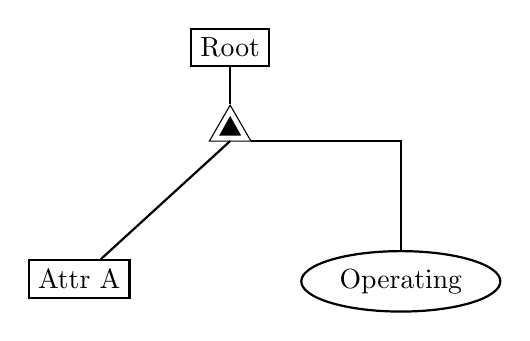
\begin{tikzpicture}
    %start
    \node [opmobject] (root) {Root};
    \node [opmexhibition, below=of root] (root-aggr) {};
    \path (root) edge (root-aggr.north);
    \node [opmobject, below left=of root-aggr] (part-a) {Attr A};
    \node [opmprocess, below right=of root-aggr] (part-b) {Operating};
    \path (root-aggr) edge (part-a);
    \draw [thick] (root-aggr.east) -| (part-b.north);
    %stop
  \end{tikzpicture}
\end{LTXexample}

Note that one could equally well have a Rooting process instead of
Root in exhibition.


%%% GENERALIZATION
\begin{LTXexample}[rangeprefix=\%, rangesuffix=,
  includerangemarker=false, linerange=start-stop, pos=t,
  caption=Generalization for object] 
  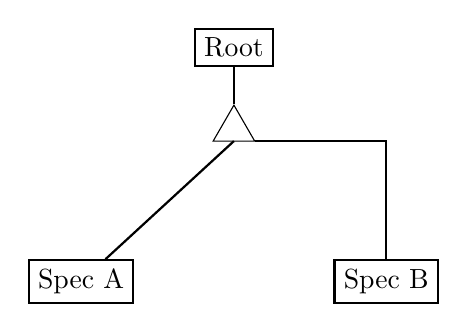
\begin{tikzpicture}
    %start
    \node [opmobject] (root) {Root};
    \node [opmgeneralization, below=of root] (root-aggr) {};
    \path (root) edge (root-aggr.north);
    \node [opmobject, below left=of root-aggr] (part-a) {Spec A};
    \node [opmobject, below right=of root-aggr] (part-b) {Spec B};
    \path (root-aggr) edge (part-a);
    \draw [thick] (root-aggr.east) -| (part-b.north);
    %stop
  \end{tikzpicture}
\end{LTXexample}

\begin{LTXexample}[rangeprefix=\%, rangesuffix=,
  includerangemarker=false, linerange=start-stop, pos=t,
  caption=Generalization for process] 
  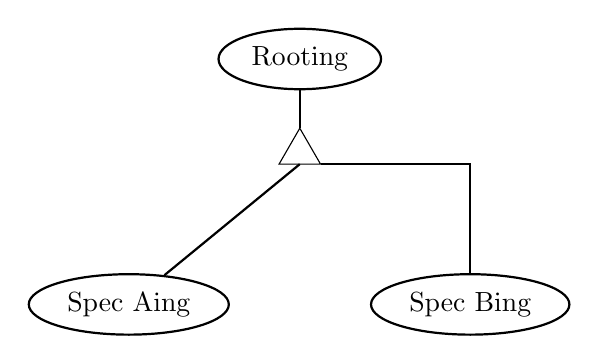
\begin{tikzpicture}
    %start
    \node [opmprocess] (root) {Rooting};
    \node [opmgeneralization, below=of root] (root-aggr) {};
    \path (root) edge (root-aggr.north);
    \node [opmprocess, below left=of root-aggr] (part-a) {Spec Aing};
    \node [opmprocess, below right=of root-aggr] (part-b) {Spec Bing};
    \path (root-aggr) edge (part-a);
    \draw [thick] (root-aggr.east) -| (part-b.north);
    %stop
  \end{tikzpicture}
\end{LTXexample}

%% INSTANTIATION
\begin{LTXexample}[rangeprefix=\%, rangesuffix=,
  includerangemarker=false, linerange=start-stop, pos=t,
  caption=Instantiation for object] 
  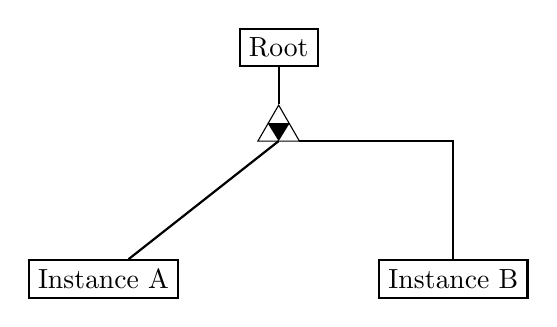
\begin{tikzpicture}
    %start
    \node [opmobject] (root) {Root};
    \node [opminstantiation, below=of root] (root-aggr) {};
    \path (root) edge (root-aggr.north);
    \node [opmobject, below left=of root-aggr] (part-a) {Instance A};
    \node [opmobject, below right=of root-aggr] (part-b) {Instance B};
    \path (root-aggr) edge (part-a);
    \draw [thick] (root-aggr.east) -| (part-b.north);
    %stop
  \end{tikzpicture}
\end{LTXexample}

\begin{LTXexample}[rangeprefix=\%, rangesuffix=,
  includerangemarker=false, linerange=start-stop, pos=t,
  caption=Instantiation for process] 
  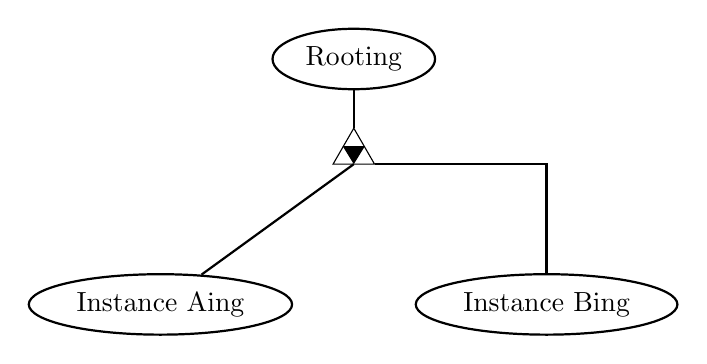
\begin{tikzpicture}
    %start
    \node [opmprocess] (root) {Rooting};
    \node [opminstantiation, below=of root] (root-aggr) {};
    \path (root) edge (root-aggr.north);
    \node [opmprocess, below left=of root-aggr] (part-a) {Instance Aing};
    \node [opmprocess, below right=of root-aggr] (part-b) {Instance Bing};
    \path (root-aggr) edge (part-a);
    \draw [thick] (root-aggr.east) -| (part-b.north);
    %stop
  \end{tikzpicture}
\end{LTXexample}

\begin{LTXexample}[rangeprefix=\%, rangesuffix=,
  includerangemarker=false, linerange=start-stop, pos=t,
  caption=Consumption] 
  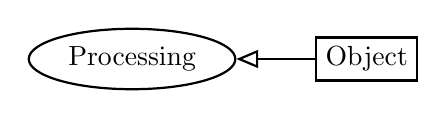
\begin{tikzpicture}
    %start
    \node [opmprocess] (processing) {Processing};
    \node [opmobject, right=of processing] (object) {Object};
    \path (processing) edge[opmconsumes] (object);
    %stop
  \end{tikzpicture}
\end{LTXexample}

\begin{LTXexample}[rangeprefix=\%, rangesuffix=,
  includerangemarker=false, linerange=start-stop, pos=t,
  caption=Result] 
  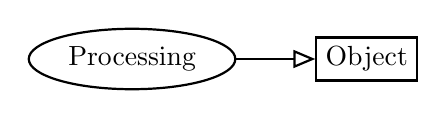
\begin{tikzpicture}
    %start
    \node [opmprocess] (processing) {Processing};
    \node [opmobject, right=of processing] (object) {Object};
    \path (processing) edge[opmyields] (object);
    %stop
  \end{tikzpicture}
\end{LTXexample}

\begin{LTXexample}[rangeprefix=\%, rangesuffix=,
  includerangemarker=false, linerange=start-stop, pos=t,
  caption=Effect] 
  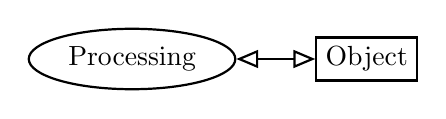
\begin{tikzpicture}
    %start
    \node [opmprocess] (processing) {Processing};
    \node [opmobject, right=of processing] (object) {Object};
    \path (processing) edge[opmaffects] (object);
    %stop
  \end{tikzpicture}
\end{LTXexample}

\begin{LTXexample}[rangeprefix=\%, rangesuffix=,
  includerangemarker=false, linerange=start-stop, pos=t,
  caption=Agent] 
  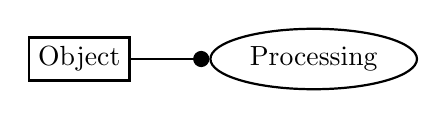
\begin{tikzpicture}
    %start
    \node [opmprocess] (processing) {Processing};
    \node [opmobject, left=of processing] (object) {Object};
    \path (object) edge[opmhandles] (processing);
    %stop
  \end{tikzpicture}
\end{LTXexample}

\begin{LTXexample}[rangeprefix=\%, rangesuffix=,
  includerangemarker=false, linerange=start-stop, pos=t,
  caption=Instrument] 
  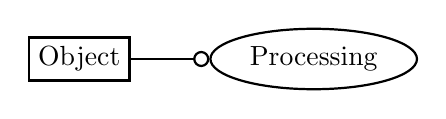
\begin{tikzpicture}
    %start
    \node [opmprocess] (processing) {Processing};
    \node [opmobject, left=of processing] (object) {Object};
    \path (processing) edge[opmrequires] (object);
    %stop
  \end{tikzpicture}
\end{LTXexample}

\begin{LTXexample}[rangeprefix=\%, rangesuffix=,
  includerangemarker=false, linerange=start-stop, pos=t,
  caption=Invocation] 
  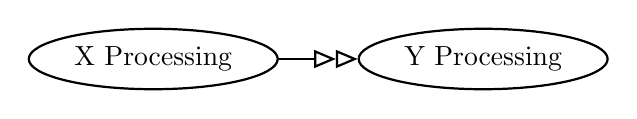
\begin{tikzpicture}
    %start
    \node [opmprocess] (x-processing) {X Processing};
    \node [opmprocess, right=of x-processing] (y-processing) {Y Processing};
    \path (x-processing) edge[opminvokes] (y-processing);
    %stop
  \end{tikzpicture}
\end{LTXexample}

Note that the version with two arrow heads have been chosen since it
is easier to work with than with the lightning zig-zag line that OPM
uses in the book.

\begin{LTXexample}[rangeprefix=\%, rangesuffix=,
  includerangemarker=false, linerange=start-stop, pos=t,
  caption=State] 
  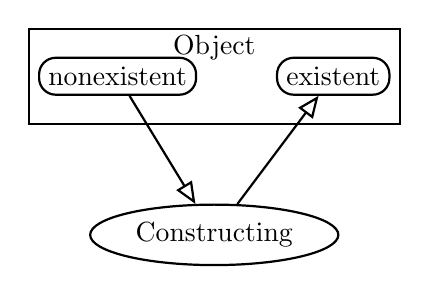
\begin{tikzpicture}
    %start
    \node [opmstate] (nonexistent) {nonexistent};
    \node [opmstate, right=of nonexistent] (existent) {existent};
    \node [opmobject, fit=(nonexistent) (existent), text depth=5ex] (object) {Object};

    \node [opmprocess, below=of object] (constructing) {Constructing};
    \path (constructing) edge[opmconsumes] (nonexistent);
    \path (constructing) edge[opmyields] (existent);
    %stop
  \end{tikzpicture}
\end{LTXexample}

This is not optimal, so I could do with some help on making this
drawing nicer. Using \verb|text depth=5ex| is a very crude way of scaling the object
box. Putting the \verb|text depth| inside a Tikz style does not help
\emph{unless} one ensures that it is called after the \verb|fit| key.

\end{document}


%%% Local Variables: 
%%% mode: latex
%%% TeX-master: t
%%% End: 
